\documentclass[xcolor = table]{beamer}

% file: preamble.tex

\usepackage{xeCJK}
\usepackage{zhnumber}	% counters in Chinese
\usepackage{fontspec}
\usepackage{comment}
\usepackage{xifthen}
\usepackage{verbatim}

\usetheme{CambridgeUS} % try Madrid
\usecolortheme{beaver} % try beaver, dolphin, seahorse
% \usefonttheme[onlymath]{serif} % try "professionalfonts"
\usefonttheme{serif}  % standard font (same with that in ``standalone'')
% \setCJKmainfont{Microsoft YaHei} % try SimSun

\usepackage{amsmath, amsfonts, amssymb, mathtools, pifont}
\newcommand{\cmark}{\ding{51}}%
\newcommand{\xmark}{\ding{55}}%
\def\checkmark{\tikz\fill[scale=0.5](0,.35) -- (.25,0) -- (1,.7) -- (.25,.15) -- cycle;} 

\usepackage[normalem]{ulem} % strike through text
\newcommand{\soutthick}[1]{%
    \renewcommand{\ULthickness}{2.0pt}%
       \sout{#1}%
    \renewcommand{\ULthickness}{.4pt}% Resetting to ulem default
}

\setbeamersize{text margin left = 2em, text margin right = 1em}
\setbeamercolor{footnote mark}{fg = teal}
\setbeamertemplate{itemize items}[default]
\setbeamertemplate{enumerate items}[default]

% \hypersetup{colorlinks = false, urlcolor = DarkRed}

% \usepackage{perpage} %the perpage package
% \MakePerPage{footnote} %the perpage package command

\usepackage{tikz}
\usepackage{pgfplots}
\usetikzlibrary{arrows.meta, shapes, positioning, calc, chains, backgrounds, fit, mindmap, intersections}

\newcommand*{\circled}[2][]{\tikz[baseline=(C.base)]{
    \node[inner sep = 0pt] (C) {\vphantom{1g}#2};
    \node[draw, circle, inner sep = 3pt, yshift = 1pt, fill = red!40, opacity = 0.5]
        at (C.center) {\vphantom{1g}};}}

\theoremstyle{plain}
\newtheorem{cdef}{定义}[section]
\newtheorem{ctheorem}{定理}[section]
\newtheorem{clemma}{引理}[section]
\newtheorem{cquestion}{问题:}[section]
\newtheorem{cobservation}{观察}[section]
\newtheorem{prop}{命题}
\theoremstyle{proof}
\newtheorem{cproof}{证明}[section]

% for tables
\usepackage{multirow}
\newcommand{\innercell}[2]{\begin{tabular}{@{}#1@{}}#2\end{tabular}}
\usepackage{hhline}
%%%%%%%%%%%%%% for appendix %%%%%%%%%%%%%%%%
% http://www-ljk.imag.fr/membres/Jerome.Lelong/latex/appendixnumberbeamer.sty
% Reference: http://tex.stackexchange.com/questions/2541/beamer-frame-numbering-in-appendix
\usepackage{appendixnumberbeamer}
% Add total frame count to slides, optional. From Stefan,
% http://www.latex-community.org/forum/viewtopic.php?f=4&t=2173
\expandafter\def\expandafter\insertshorttitle\expandafter{%
  \insertshorttitle\hfill\insertframenumber\,/\,\inserttotalframenumber}
%%%%%%%%%%%%%% for appendix %%%%%%%%%%%%%%%%
\usepackage{graphicx, subcaption}

\usepackage{caption}
\DeclareCaptionLabelSeparator{none}{}
\captionsetup{labelsep = none}

\makeatletter
\let\@@magyar@captionfix\relax
\makeatother

\usepackage[export]{adjustbox}
% for fig without caption: #1: width/size; #2: fig file
\newcommand{\fignocaption}[2]{
  \begin{figure}[htp]
    \centering
    \includegraphics[#1]{#2}
  \end{figure}
}

% for fig without caption: #1: width/size; #2: fig file; #3: fig caption
\newcommand{\fig}[3]{
  \begin{figure}[htp]
    \centering
      \includegraphics[#1]{#2}
      \caption{#3}
  \end{figure}
}

% colors
\definecolor{DarkRed}{rgb}{0.55, 0.0, 0.0}
\newcommand{\red}[1]{\textcolor{red}{#1}}
\newcommand{\redoverlay}[2]{\textcolor<#2>{red}{#1}}
\newcommand{\green}[1]{\textcolor{green}{#1}}
\newcommand{\greenoverlay}[2]{\textcolor<#2>{green}{#1}}
\newcommand{\blue}[1]{\textcolor{blue}{#1}}
\newcommand{\blueoverlay}[2]{\textcolor<#2>{blue}{#1}}
\newcommand{\purple}[1]{\textcolor{purple}{#1}}
\newcommand{\cyan}[1]{\textcolor{cyan}{#1}}
\newcommand{\violet}[1]{\textcolor{violet}{#1}}
\newcommand{\lgray}[1]{\textcolor{lightgray}{#1}}
\newcommand{\teal}[1]{\textcolor{teal}{#1}}
\newcommand{\brown}[1]{\textcolor{brown}{#1}}

\newcommand{\wlspec}{$\mathcal{A}_{\text{weak}}$}

% colorded box
\newcommand{\rbox}[1]{\red{\boxed{#1}}}
\newcommand{\gbox}[1]{\green{\boxed{#1}}}
\newcommand{\bbox}[1]{\blue{\boxed{#1}}}
\newcommand{\pbox}[1]{\purple{\boxed{#1}}}

\usepackage[linewidth = 1pt, framemethod = TikZ]{mdframed}
\mdfsetup{frametitlealignment=\center}

\newcommand{\hl}[1]{\fcolorbox{yellow}{yellow!60}{#1}}

% for cite: #1: author; #2: conference #3: year
\newcommand{\citeinbeamer}[3]{{\tiny{\textcolor{blue}{[#1@#2'#3]}}}}

\usepackage[natbib = true, backend = bibtex, style = authoryear]{biblatex}
\setbeamertemplate{bibliography item}[article]
\renewcommand*{\bibfont}{\footnotesize}
\addbibresource{njucs-youth-salon-2018-report.bib}

\newcommand{\ncite}[1]{\violet{\footnotesize [\cite{#1}]}}

\newcommand{\term}[1]{\small (#1)}
\newcommand{\set}[1]{\{#1\}}
\newcommand{\question}[1]{\textcolor{red}{\centerline{#1}}}
\newcommand{\answer}[1]{\textcolor{blue}{\centerline {#1}}}
\newcommand{\alertred}[1]{\textcolor{red}{#1}}
\newcommand{\alertblue}[1]{\textcolor{blue}{#1}}
\newcommand{\todo}[1]{\textcolor{red}{\textbf{TODO:} #1}}
\newcommand{\mathbfblue}[1]{\textcolor{blue}{$\mathbf{#1}$}}

\newcommand{\hhref}[2]{\centerline{\href{#1}{\purple{\underline{#2}}}}}

\newcommand{\papertitle}{复制数据类型理论研究}

\newcommand{\thankyou}{
  \begin{frame}{}
    \begin{columns}
      \column{0.50\textwidth}
	\fignocaption{width = 0.80\textwidth}{figs/rdt-research-two-work}
      \column{0.50\textwidth}
	\fignocaption{width = 0.80\textwidth}{figs/thankyou}
    \end{columns}

    \begin{columns}[b]
      \column{0.30\textwidth}
	\fignocaption{width = 0.90\textwidth}{figs/hfwei-mail}
	\vspace{-0.20cm}
	\hhref{http://www.bigoh.net/wiki/index.php/user:Hengfeng-Wei}{hengxin@homepage}
      \column{0.30\textwidth}
	\fignocaption{width = 0.50\textwidth}{figs/github-icon}
	\vspace{-0.20cm}
	\hhref{https://github.com/hengxin}{hengxin@github}
      \column{0.30\textwidth}
	\fignocaption{width = 0.80\textwidth}{figs/hengxin-stack}
	\vspace{-0.20cm}
	\hhref{https://stackexchange.com/users/2055160/hengxin}{hengxin@stackexchange}
    \end{columns}
  \end{frame}
}

%%%%%%%%%%%%%%%%%%%%%%%%%%%%%%%%%%%%%%%%%%%%%%%%%%%%%%%%%%%%%%%%%%%%%%%%%%%%%%%%	
\title[复制数据类型]{\papertitle}
\subtitle{(青年学者学术沙龙)}

\author[魏恒峰]{魏恒峰}
\titlegraphic{
\includegraphics[height = 1.3cm]{figs/nju-logo-purple}~
\includegraphics[height = 1.3cm]{figs/cs-logo}}
\institute{南京大学软件所}
% \date{\zhtoday}
\date{2018年12月21日}

% Comment this, if you do not want the table of contents to pop up 
% at the beginning of each section: 
% \AtBeginSection[]{
%   \begin{frame}[noframenumbering, plain]
%     \frametitle{\papertitle}
%     \tableofcontents[currentsection, sectionstyle=show/shaded, subsectionstyle=hide/hide/hide]
%   \end{frame}
% }

% Comment this, if you do not want the table of contents to pop up 
% at the beginning of each subsection:
% \AtBeginSubsection[]{
%   \begin{frame}[noframenumbering, plain]
%     \frametitle{\papertitle}
%       \tableofcontents[currentsection, sectionstyle=show/shaded, subsectionstyle=show/shaded/hide]
%   \end{frame}
% }
%%%%%%%%%%%%%%%%%%%%
\begin{document}

\renewcommand\figurename{} % no ``图''
\renewcommand\tablename{}  % no ``表''

% mdf: mdframed; #1: frame color; #2: frame title color; #3: frame title; #4: text
\newcommand{\mdf}[4]{
\begin{mdframed}[frametitle={
  \tikz[baseline = (current bounding box.east), outer sep = 0pt]
  \node[anchor = east, rectangle, fill = #1!20, font = \small]{\strut \textcolor{#2}{#3}};},
  innertopmargin = 2pt, linecolor = #1!20, linewidth = 2pt, topline = true,
  frametitleaboveskip=\dimexpr-\ht\strutbox\relax]
  #4
\end{mdframed}
}

\maketitle

% file: sections/intro.tex

\section{研究背景}

%%%%%%%%%%%%%%%
\begin{frame}{}
  \begin{center}
    {\large Abstract Data Types} \ncite{Liskov:VHLL74} \\[8pt]

    (单线程; 顺序语义)
  \end{center}

  \begin{columns}
    \column{0.40\textwidth}
      \fignocaption{width = 0.60\textwidth}{figs/alg-ds-wirth}
    \pause
    \column{0.40\textwidth}
      \fignocaption{width = 0.25\textwidth}{figs/adt}
  \end{columns}
\end{frame}
%%%%%%%%%%%%%%%

%%%%%%%%%%%%%%%
\begin{frame}{}
  \begin{center}
    {\large Concurrent Data Types} \ncite{Herlihy:TOPLAS90} \\[8pt]

    (多线程; 并发语义)
  \end{center}

  \begin{columns}
    \column{0.40\textwidth}
      \fignocaption{width = 0.70\textwidth}{figs/taomp-herlihy}
    \pause
    \column{0.50\textwidth}
      \fignocaption{width = 0.45\textwidth}{figs/cdt}

      \only<3->{
	\begin{center}
	  \hl{\Large PL} {(Programming Language)}
	\end{center}
      }
  \end{columns}
\end{frame}
%%%%%%%%%%%%%%%

%%%%%%%%%%%%%%%
\begin{frame}{}
  \begin{center}
    \hl{\large Replicated Data Types} \ncite{Shapiro:TR11} \ncite{Burckhardt:POPL14} \\[8pt]

    (多副本; 复制语义)
  \end{center}

  \pause
  \fignocaption{width = 0.30\textwidth}{figs/rdt}

  \pause
  \begin{center}
    \hl{\Large DC} {(Distributed Computing)}
  \end{center}
\end{frame}
%%%%%%%%%%%%%%%

%%%%%%%%%%%%%%%
% \begin{frame}{}
%   \begin{columns}
%     \column{0.50\textwidth}
%       \fignocaption{width = 0.60\textwidth}{figs/keep-calm-why-bother}
%     \pause
%     \column{0.50\textwidth}
%       \centerline{\hl{\red{\Huge 新平台}}}
%   \end{columns}
% \end{frame}
%%%%%%%%%%%%%%%

%%%%%%%%%%%%%%%
\begin{frame}{}
  \begin{center}
    {\hl{\Large 新平台: 大规模分布式系统}}
  \end{center}

  \fignocaption{width = 0.50\textwidth}{figs/sina-weibo-world-map.pdf}

  \pause
  \vspace{0.10cm}
  \begin{center}
    低延迟 \quad 高可用性 {\small (4个9)} \quad 高容错性 \quad 高可扩展性
  \end{center}

  % \begin{columns}
  %   \column{0.40\textwidth}
  %   新浪微博社交应用~\footnotemark:
  %   \begin{itemize}
  %     \item 日均用户近一亿名
  %     \item 日均消息近一亿条
  %   \end{itemize}
  %   \pause
  %   \column{0.50\textwidth}
  %   特性需求: 
  %   \begin{itemize}
  %     \item 低延迟, 高可用性 (4个9~\footnotemark)
  %     \item 高容错性, 高可扩展性
  %   \end{itemize}
  % \end{columns}
  % 
  % \footnotetext[1]{2015第三季度; 数据来自 \href{https://www.chinainternetwatch.com/15740/weibo-q3-2015/}{China Internet Watch}.}
  % % See http://tex.stackexchange.com/a/340079/23098
  % \alt<1>{\let\thefootnote\relax\footnotetext{~}}{\footnotetext[2]{数据来自 \href{http://www.infoq.com/cn/articles/weibo-platform-availability-9999}{InfoQ}.}}
\end{frame}
%%%%%%%%%%%%%%%
\begin{frame}{}
  \graphicspath{{tikz/}}
  \begin{figure}[h!]
    \centering
    \begin{adjustbox}{max totalsize = {0.50\textwidth}{1.00\textheight}, center}
      % File: beamer overlay for distributed-data.tex
% Created: July 23, 2016

\begin{tikzpicture}[rc/.style = {circle, minimum size = 4cm, fill = red},
  br/.style = {rectangle, rounded corners, minimum size = 4cm, fill = blue},
  gs/.style = {shape = star, scale = 8, star points = 5, star point ratio = 1.65, fill = green},
  dash pattern = {on 20pt off 10pt},
  partition/.style = {draw, lightgray, line width = 8pt},
  replication/.style = {draw, dash phase = 0pt, line width = 10pt, #1},
  access/.style = {draw, > = stealth, <->, dash phase = 0pt, line width = 6pt, brown}]

  \uncover<1->{
  \begin{pgfonlayer}{background}
	\node[opacity = 0.80] (map) {\includegraphics[scale = 0.50]{figs/world-map-logo.jpg}};
  \end{pgfonlayer}

  % shared data
  \begin{scope}[yshift = -18cm]
	\node[rc] (circ) {};
	\node[br, left = 2cm of circ] (rect) {};
	\node[gs, right = 2cm of circ] (st) {};

	\begin{pgfonlayer}{background}
	  \node[rectangle, rounded corners, fill = black!30, fit = (circ) (rect) (st), inner sep = 5pt, 
		label = {[font = \fontsize{65}{70}\sffamily\bfseries] below : Application Data}] (data) {};
	\end{pgfonlayer}
  \end{scope}
  }

  \uncover<2->{
  % partition
  \node[rc] (circ1) at (20, 10) {};
  \node[br] (rect1) at (-25, 10) {};
  \node[gs] (st1) at (28, -12) {};

  \draw[partition] (circ) to (circ1);
  \draw[partition] (rect) to (rect1);
  \draw[partition] (st) to (st1);
  }

  \uncover<3->{
  % replication
  \node[rc] (circ2) at (-15, -10) {};
  \node[rc] (circ3) at (-10, 18) {};

  \node[br] (rect2) at (10, 12) {};

  \node[gs] (st2) at (0,0) {};
  \node[gs] (st3) at (20, 5) {};

  \path[replication = {red}] (circ1) to (circ2) 
  	(circ2) to (circ3)
	(circ3) to (circ1);

  \path[replication = {blue}] (rect1) to (rect2);

  \path[replication = {green}] (st1) to (st2) 
  	(st2) to (st3)
	(st3) to (st1);
  }

%  \uncover<5->{
%  % sina-weibo clients
%  \def\SCALE{0.15}
%  \node[] (sina1) at (-25, 0) {
\includegraphics[scale = \SCALE]{figs/sina-weibo.png}};
%  \node[] (sina2) at (10, 5) {
\includegraphics[scale = \SCALE]{figs/sina-weibo.png}};
%  \node[] (sina3) at (5, -10) {
\includegraphics[scale = \SCALE]{figs/sina-weibo.png}};
%
%  % access
%  \path[every edge/.append style = {access}] (sina1) edge (rect1)
%  				(sina1) edge (circ2)
%				(sina2) edge (rect2)
%				(sina2) edge (st2)
%				(sina3) edge (circ1)
%				(sina3) edge (st2);
%  }
\end{tikzpicture}

    \end{adjustbox}
  \end{figure}

  \vspace{0.20cm}
  \begin{center}
    \begin{minipage}{0.65\textwidth}
      \red{\large 分布数据 \term{distributed data}:}

      \vspace{0.20cm}
      \begin{enumerate}
	\item<2-> 分区 \term{partition}: 水平扩展
	\item<3-> \hl{副本 \term{replication}}: 就近访问, 容灾备份
      \end{enumerate}
    \end{minipage}
  \end{center}
\end{frame}
%%%%%%%%%%%%%%%

%%%%%%%%%%%%%%%
\begin{frame}{}
  \begin{center}
    \begin{minipage}{0.50\textwidth}
      {\large 复制数据类型} \ncite{Shapiro:TR11} 

      \vspace{0.20cm}
      \begin{itemize}
	\setlength{\itemsep}{4pt}
	\item Read/Write Register
	\item Counter
	\item Set
	\item List
	\item HashMap
	\item Disjoint Set
	\item Graph
	\item $\dots$
      \end{itemize}
    \end{minipage}
  \end{center}
\end{frame}
%%%%%%%%%%%%%%%

%%%%%%%%%%%%%%%
\begin{frame}{}
  \begin{columns}
    \column{0.40\textwidth}
      \fignocaption{width = 0.98\textwidth}{figs/what-is-new}
    \column{0.60\textwidth}
      \centerline{\hl{\red{\Huge 新问题, 新挑战}}}
  \end{columns}

  \pause
  \vspace{0.30cm}
  \fignocaption{frame, width = 0.80\textwidth}{figs/rdt-popl}
  \centerline{\ncite{Burckhardt:POPL14}}
\end{frame}
%%%%%%%%%%%%%%%

%%%%%%%%%%%%%%%
\begin{frame}{}
  \begin{center}
    \resizebox{0.65\textwidth}{!}{% file: rdt-research-two-work.tex

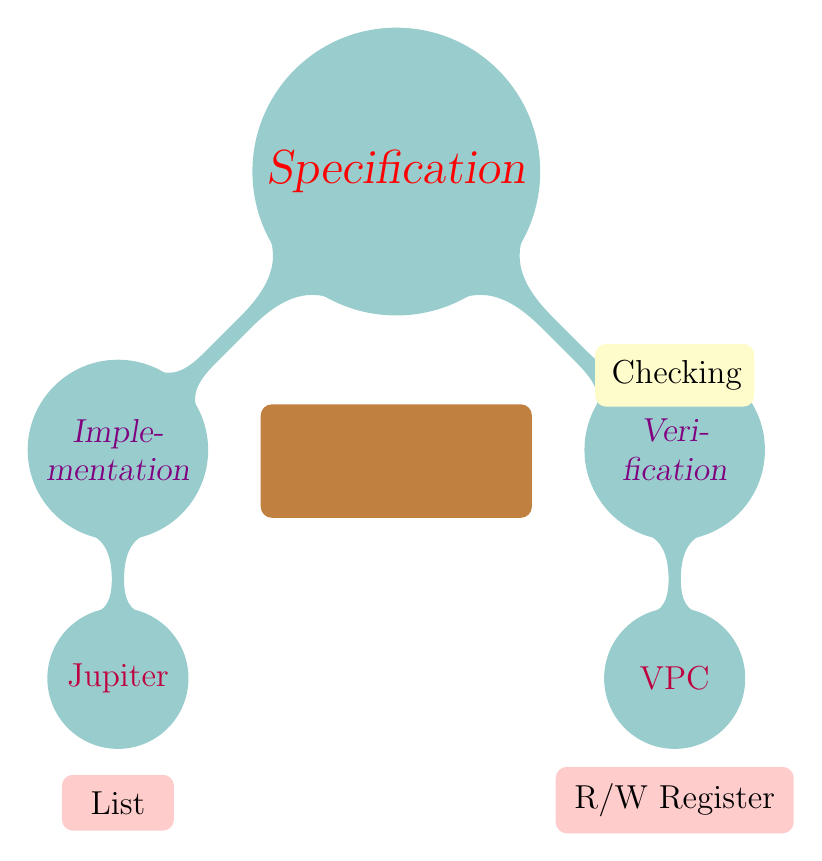
\begin{tikzpicture}[
    root concept/.append style = {concept color = teal!40, sibling angle = 90, font = \LARGE, minimum size = 0pt, red},
    level 1 concept/.append style = {concept color = teal!40, sibling angle = 90, font = \large, violet},
    level 2 concept/.append style = {concept color = teal!40, font = \large, purple},
    every annotation/.style = {fill = red!20, font = \sf, align = center, font = \large,
      minimum size = 5pt, inner sep = 6pt, text width = 2.6cm}
  ] 
  \path[mindmap]
    node (spec) [concept] {\textsl{Specification}}
    [counterclockwise from = 225]

    child[] {
      node (impl) [concept] {\textsl{Imple\-mentation}}
      [counterclockwise from = -90]
      child { node (jupiter) [concept, font = \large] {Jupiter} }
    }
    child[] {
      node (veri) [concept] {\textsl{Veri\-fication}}
      [clockwise from = -90]
      child { node (vpc) [concept, font = \large] {VPC} }
    };

    \uncover<2->{\node [annotation, below = 0.20cm of jupiter.south, text width = 1.0cm] {List};}
    \uncover<3->{\node [annotation, below = 0.10cm of vpc.south] {R/W Register};}
    \uncover<4->{\node [annotation, fill = yellow!20, above = 0.40cm of veri.center, text width = 1.6cm] {Checking};}

    \node [annotation, fill = brown!20, below = 1.00cm of spec.south, font = \Huge, inner sep = 12pt, brown] {RDT};
\end{tikzpicture}
}
  \end{center}
\end{frame}
%%%%%%%%%%%%%%%

% file: sections/work

\section{两份工作}

%%%%%%%%%%%%%%%%%%%%%%%%%

%%%%%%%%%%%%%%%
% file: sections/jupiter.tex

\subsection{Jupiter: 实现与正确性证明}

%%%%%%%%%%%%%%%
\begin{frame}{}
  \fignocaption{width = 0.65\textwidth}{figs/rdt-research-jupiter}
\end{frame}
%%%%%%%%%%%%%%%

% file: sections/jupiter-work.tex

%%%%%%%%%%%%%%%%%%%%
\begin{frame}{}
  \begin{center}
    \begin{mdframed}[frametitle = {\large 复制列表数据类型~\footnotemark}, frametitlerule = true, frametitlebackgroundcolor = brown!20,
      frametitleaboveskip = 8pt, frametitlebelowskip = 8pt, innertopmargin = 10pt]
      {\large 实现复制列表的 \blue{Jupiter 协议}~\ncite{Nichols:UIST95}\footfullcite{Nichols:UIST95} \red{满足} \\
      \blue{weak list specification}~\ncite{Attiya:PODC16}\footfullcite{Attiya:PODC16}.} \\[15pt]
    \end{mdframed}

    \footnotetext{\normalsize \uncover<2->{藏在脚注里的}\red{猜想}@PODC'2016~\ncite{Attiya:PODC16}}
  \end{center}
\end{frame}
%%%%%%%%%%%%%%%%%%%%

%%%%%%%%%%%%%%%%%%%%
\begin{frame}{}
  \fignocaption{width = 0.30\textwidth}{figs/outline}
  \begin{center}
    \hl{\large 提纲}
  \end{center}

  \pause
  \begin{columns}
    \column{0.60\textwidth}
      \begin{enumerate}[<+->]
	\setlength{\itemsep}{12pt}
	\item 为什么要研究复制列表数据类型?
	\item 什么是 \red{weak list specification} \wlspec{}?
	\item \red{Jupiter} 协议是如何工作的?
	\item 如何证明Jupiter满足\wlspec{}?
      \end{enumerate}
  \end{columns}
\end{frame}
%%%%%%%%%%%%%%%%%%%%

%%%%%%%%%%%%%%%%%%%%
\begin{frame}{}
  \centerline{\teal{\Large 基于\red{副本}的协同文本编辑系统}}

  % \vspace{-0.20cm}
  \fignocaption{width = 0.55\textwidth}{figs/coeditor}

  \pause
  \vspace{-0.40cm}
  \begin{center}
    \begin{itemize}
      \centering
      \item 副本节点要\red{立即}响应本地用户操作 \\[4pt]
      \item 更新操作\red{异步}传播到其它副本节点
    \end{itemize}
  \end{center}
\end{frame}
%%%%%%%%%%%%%%%%%%%%

%%%%%%%%%%%%%%%%%%%%
\begin{frame}{}
  \centerline{\Large \red{复制列表对象}: 建模编辑系统的核心功能}
  \vspace{0.30cm}

  \begin{center}
    \begin{minipage}{0.70\textwidth}
      \begin{description}
	\setlength{\itemsep}{10pt}
	\item[$\textsc{Ins}(a, p):$] 在 $p$ 位置插入元素 $a$
	\item[$\textsc{Del}(p):$] 删除 $p$ 位置上的元素
	\item[$\textsc{Read}:$] 返回该列表
      \end{description}
    \end{minipage}
  \end{center}
\end{frame}
%%%%%%%%%%%%%%%%%%%%

%%%%%%%%%%%%%%%%%%%%
\begin{frame}{}
  \begin{cdef}[最终收敛性 (Eventual Convergence)~\ncite{Ellis:SIGMOD89}]
    当系统处于``静默'' \teal{\emph{(Quiescence)}} 状态时, 所有副本节点上的列表是相同的。
  \end{cdef}

  \vspace{0.30cm}
  \begin{cdef}[强最终一致性 (Strong Eventual Consistency)~\ncite{Shapiro:SSS11}]
    如果两个副本节点处理了同一组更新操作, 则它们的列表是相同的。
  \end{cdef}

  \pause
  \vspace{0.60cm}
  \centerline{\red{\large 对系统的\red{中间状态}缺少足够的约束}}
\end{frame}
%%%%%%%%%%%%%%%%%%%%

%%%%%%%%%%%%%%%%%%%%
\begin{frame}{}
  \fignocaption{width = 0.80\textwidth, frame}{figs/podc16-attiya}

  \vspace{0.20cm}
  \begin{cdef}[Weak List Specification \wlspec{}~\ncite{Attiya:PODC16}]
    Informally, \wlspec{} requires the ordering between \red{elements that are not deleted} to be consistent across the system.
  \end{cdef}

  \vspace{0.60cm}
  \centerline{\teal{\large 定义在系统所有列表状态上的\red{全局}性质}}
\end{frame}
%%%%%%%%%%%%%%%%%%%%

%%%%%%%%%%%%%%%%%%%%
\begin{frame}{}
  \begin{center}
    {\large \wlspec{} 等价于:}
  \end{center}

  \begin{cdef}[\hl{状态对兼容性} (Pairwise State Compatibility Property)]
    任给两个列表状态 $\sigma_0$、$\sigma_1$, 若它们含有两个共同元素 $a$、$b$, \\
    则 $a$、$b$ 在 $\sigma_0$ 与 $\sigma_1$ 中的相对顺序保持一致。
  \end{cdef}

  \vspace{0.30cm}
  \begin{columns}
    \column{0.50\textwidth}
      \fignocaption{width = 0.50\textwidth}{figs/ex-weak-list-spec}
      \vspace{-0.60cm}
      \fignocaption{width = 0.30\textwidth}{figs/red-cross}
    \pause
    \column{0.50\textwidth}
      \fignocaption{width = 0.65\textwidth}{figs/ex-strong-list-spec}
      \vspace{-0.60cm}
      \fignocaption{width = 0.20\textwidth}{figs/green-check}
      \vspace{-1.20cm}
      \uncover<3->{
	\begin{center}
	  \red{\footnotesize ``Strong List Specification''不允许}
	\end{center}
      }
  \end{columns}
\end{frame}
%%%%%%%%%%%%%%%%%%%%

%%%%%%%%%%%%%%%%%%%%
\begin{frame}{}
  \centerline{\Huge \teal{Jupiter}}
\end{frame}
%%%%%%%%%%%%%%%%%%%%

%%%%%%%%%%%%%%%%%%%%
\begin{frame}{}
  \centerline{\large $\blue{(n+1)}\; \text{replicas} \triangleq \blue{(n)}\; \text{\red{Client}} + \blue{(1)}\; \text{\red{Server}}$~\ncite{Nichols:UIST95}}

  \begin{center}
    \resizebox{0.50\textwidth}{!}{\input{tikz/jupiter-cs-tikz}}
  \end{center}

  \vspace{-0.60cm}
  \uncover<2->{
    \begin{center}
      \red{Server 负责将所有操作序列化} \\[6pt]
      用户操作 $\xrightarrow[\text{\hl{立即返回}}]{\quad \text{提交} \quad}$ Client 
      $\xrightarrow[\text{更新操作}]{\quad \text{FIFO} \quad}$ Server $\xrightarrow[\text{更新操作}]{\quad \text{FIFO} \quad}$ 其它Clients 
    \end{center}
  }
\end{frame}
%%%%%%%%%%%%%%%%%%%%

%%%%%%%%%%%%%%%%%%%%
\begin{frame}{}
  \begin{center}
    {\large \red{挑战:} \hl{如何处理并发操作带来的冲突?}} \\[3pt] \pause
    {\small \teal{(The server is not drawn.)}}
  \end{center}

  \vspace{-0.80cm}
  \begin{columns}
    \column{0.40\textwidth}
      \begin{center}
	\input{tikz/no-ot-tcs06-tikz}
      \end{center}
    \column{0.40\textwidth}
      \begin{center}
	\input{tikz/ot-tcs06-tikz}
      \end{center}
  \end{columns}

  \vspace{-0.30cm}
  \begin{center}
    \uncover<5->{\large \red{解决方案:} \hl{操作转换} (Operational Transformation; OT)\\\ncite{Ellis:SIGMOD89}}
  \end{center}
\end{frame}
%%%%%%%%%%%%%%%%%%%%

%%%%%%%%%%%%%%%%%%%%
\begin{frame}{}
  \fignocaption{width = 0.40\textwidth}{figs/ot}

  \begin{equation*}
    \text{\hl{交换律:}}\;\; \resizebox{0.35\textwidth}{!}{$\sigma; o_1; o_2' \equiv \sigma; o_2; o_1'$}
  \end{equation*}

  \centerline{\ncite{Ellis:SIGMOD89}}
\end{frame}
%%%%%%%%%%%%%%%%%%%%

%%%%%%%%%%%%%%%%%%%%
\begin{frame}{}
  \begin{center}
    \red{\large 问题: 如果副本节点之间偏离 \teal{\small (diverge)} 多个 ($\ge 2$) 操作, 怎么办?} \\[8pt]

    \resizebox{0.75\textwidth}{!}{\input{tikz/ot-diverge-two}}
  \end{center}
\end{frame}
%%%%%%%%%%%%%%%%%%%%

%%%%%%%%%%%%%%%%%%%%
\begin{frame}{}
  \begin{center}
    \hl{核心问题:} \\[8pt]
    当副本节点$r$接收到由Server转发的操作$o$时,\\
    如何对$o$执行操作转换?
  
    \pause
    \vspace{0.80cm}
    \red{\large 与哪些操作进行转换?以什么顺序进行转换?}

    \pause
    \vspace{0.80cm}

    \hl{核心思想:} \\[3pt]
    \begin{columns}
      \column{0.72\textwidth}
	\begin{enumerate}
	  \item 与``$r$ 上已执行且与 $o$ \purple{并发}的操作''进行转换
	  \item 以``由 Server 确定的\purple{序列化}顺序''进行转换 
	\end{enumerate}
    \end{columns}
  \end{center}
\end{frame}
%%%%%%%%%%%%%%%%%%%%

%%%%%%%%%%%%%%%%%%%%
\begin{frame}{}
  \begin{center}
    {\large 利用数据结构 \hl{$2D$ 状态空间}~\ncite{Xu:CSCW14} \\
    控制何时以及如何执行``操作转换''}
  \end{center}

  \fignocaption{width = 0.60\textwidth}{figs/ot-diverge-two}

  \begin{center}
    $2D$: {\textsc{Local}} \emph{vs.} \textsc{Global}
  \end{center}
\end{frame}
%%%%%%%%%%%%%%%%%%%%

%%%%%%%%%%%%%%%%%%%%
\begin{frame}{}
  \centerline{\large 每个 \red{Client} 维护一个 $2D$ 状态空间}

  \fignocaption{width = 0.70\textwidth}{figs/jupiter-illustration}

  \centerline{\large \red{Server} 维护 $n$ 个 $2D$ 状态空间, 与 $n$ 个 Clients 对应}
\end{frame}
%%%%%%%%%%%%%%%%%%%%

%%%%%%%%%%%%%%%%%%%%
\begin{frame}{}
  \begin{center}
    \hl{\Huge Mismatch!}

    \vspace{1.00cm}
    {\large \blue{\wlspec{}} 所规定的\red{全局性质}}

    \vspace{0.20cm}
    \fignocaption{width = 0.40\textwidth}{figs/mismatch}
    \vspace{0.20cm}

    {\large \blue{Jupiter} 协议中, 每个副本节点所维护的\red{局部视图}}
  \end{center}
\end{frame}
%%%%%%%%%%%%%%%%%%%%

%%%%%%%%%%%%%%%%%%%%
\begin{frame}{}
  \centerline{\LARGE \teal{CJupiter (Compact Jupiter)}}

  \pause
  \vspace{1.0cm}
  \begin{ctheorem}[等价性]
    在相同的操作调度 \emph{\teal{\small (schedule)}} 下, 
    \emph{CJupiter} 与 \emph{Jupiter} 中的对应副本节点的行为 \emph{\teal{\small (behavior; {\small 状态序列})}} 是相同的。
  \end{ctheorem}
\end{frame}
%%%%%%%%%%%%%%%%%%%%

%%%%%%%%%%%%%%%%%%%%
\begin{frame}{}
  \begin{center}
    {\large CJupiter 为每个副本节点维护一个 \hl{\red{$n$-ary} \blue{有序}状态空间}}
  \end{center}

  \begin{center}
    \resizebox{0.40\textwidth}{!}{\input{tikz/cjupiter-allinone}}
  \end{center}

  \pause
  \begin{center} 
    每个node可以有 \red{$>2$} 条出边 \\[5pt] 
    每个node的所有出边按照其上标记操作的``序列化''顺序排成\red{全序}
  \end{center}
\end{frame}
%%%%%%%%%%%%%%%%%%%%

%%%%%%%%%%%%%%%%%%%%
\begin{frame}{}
  \begin{center}
    \begin{prop}[Compactness of CJupiter]
      {\large \emph{CJupiter} 所维护的 $(n+1)$ 个$n$-ary有序状态空间是相同的。}
    \end{prop}

    \resizebox{0.45\textwidth}{!}{\input{tikz/cjupiter-allinone-path}}

    \pause
    每个副本节点的行为对应于该状态空间中的一条\hl{\red{路径}} \\[3pt]
    \pause
    \red{单个$n$-ary有序状态空间包含了系统所有可能的状态}
  \end{center}
\end{frame}
%%%%%%%%%%%%%%%%%%%%

%%%%%%%%%%%%%%%%%%%%
\begin{frame}{}
  \centerline{\teal{\LARGE CJupiter 满足 Weak List Specification}}
\end{frame}
%%%%%%%%%%%%%%%%%%%%

%%%%%%%%%%%%%%%%%%%%
\begin{frame}{}
  \begin{center}
    {\large 关注某个$n$-ary有序状态空间, \hl{三步骤}证明\red{``状态对兼容性''}}
  \end{center}

  \fignocaption{width = 0.45\textwidth}{figs/cjupiter-allinone-path}

  \pause
  \begin{center}
    \red{反证法、数学归纳法、分情形分析法}
  \end{center}
\end{frame}
%%%%%%%%%%%%%%%%%%%%

%%%%%%%%%%%%%%%%%%%%
\begin{frame}{}
  \centerline{\circled{1} 任取两个状态节点 $v_1$和$v_2$}

  \begin{clemma}[LCA (Lowest Common Ancestor)]
    $n$-ary 有序状态空间中的任意一对状态节点都有\red{唯一的}最近公共祖先。
  \end{clemma}

  \begin{columns}
    \column{0.60\textwidth}
      \fignocaption{width = 0.50\textwidth}{figs/lca}
      \column{0.30\textwidth}
	\[
	  v_0 = \text{LCA}(v_1, v_2)
	\]
  \end{columns}
\end{frame}
%%%%%%%%%%%%%%%%%%%%

%%%%%%%%%%%%%%%%%%%%
\begin{frame}{}
  \centerline{\circled{2} 考虑从 $v_0 = \text{LCA}(v_1, v_2)$ 到 $v_1$ 和 $v_2$ 的两条路径}

  \begin{clemma}[Disjoint Paths]
    路径 $P_{v_0 \leadsto v_1}$ 上包含的操作集 $O_{v_0 \leadsto v_1}$ 与路径 $P_{v_0 \leadsto v_2}$ 上包含的操作集
    $O_{v_0 \leadsto v_2}$ 不相交。
  \end{clemma}

  \begin{columns}
    \column{0.60\textwidth}
	\fignocaption{width = 0.50\textwidth}{figs/disjoint-paths}
      \column{0.30\textwidth}
	\[
	  v_0 = \text{LCA}(v_1, v_2)
	\]
  \end{columns}
\end{frame}
%%%%%%%%%%%%%%%%%%%%

%%%%%%%%%%%%%%%%%%%%
\begin{frame}{}
  \centerline{\circled{3} 考虑两条路径上的状态}

  \begin{clemma}[Compatible Paths]
    $P_{v_0 \leadsto v_1}$ 上的任一状态 $v$ 与 $P_{v_0 \leadsto v_2}$ 上的任一状态 $v'$ 是兼容的。
  \end{clemma}

  \begin{columns}
    \column{0.60\textwidth}
	\fignocaption{width = 0.55\textwidth}{figs/compatible-paths}
      \column{0.40\textwidth}
	\[
	  v_0 = \text{LCA}(v_1, v_2)
	\]

	\pause
	\vspace{0.50cm}
	\begin{center}
	  \hl{$\therefore$ $v_1$ 和 $v_2$ 是兼容的}
	\end{center}
  \end{columns}
\end{frame}
%%%%%%%%%%%%%%%%%%%%

% file: sections/jupiter-related.tex

%%%%%%%%%%%%%%%%%%%%
\begin{frame}{}
  \centerline{\large \hl{个人体会:} 基于 OT 思想的协议晦涩难懂}

  \vspace{0.60cm}
  \begin{columns}
    \column{0.50\textwidth}
      \fignocaption{width = 0.80\textwidth}{figs/thread}
    \column{0.50\textwidth}
      \pause
      \begin{itemize}
	\setlength{\itemsep}{10pt}
	\centering
	\item 协议多种多样
	\item 经常不加证明
	\item 证明是错误的
	\item<3-> \hl{\red{勘误也是错的}}
      \end{itemize}
  \end{columns}
\end{frame}
%%%%%%%%%%%%%%%%%%%%

%%%%%%%%%%%%%%%%%%%%
\begin{frame}{}
  \begin{center}
    {\large 
      Model Checking/Theorem Proving: 使用 TLA+/TLAPS \\[5pt]
      \href{https://github.com/Disalg-ICS-NJU/tlaplus-lamport-projects/tree/master/tlaplus-projects/Hengfeng-Wei/Wei-jupiter-tla}{\purple{\underline{jupiter-tlaplus@github}}}
    }
  \end{center}

  \begin{columns}
    \column{0.30\textwidth}
      \fignocaption{width = 0.80\textwidth}{figs/tlaplus}
      \vspace{-0.50cm}
      \fignocaption{width = 0.60\textwidth}{figs/lamport}
    \pause
    \column{0.50\textwidth}
      \fignocaption{width = 1.00\textwidth}{figs/jupiter-tlaplus}
  \end{columns}
\end{frame}
%%%%%%%%%%%%%%%%%%%%



% %%%%%%%%%%%%%%%%%%%%%%%%%%%%%%%%%%%%%%%%	
\subsection{PA2AM: (2-)Atomicity 一致性维护与量化}

%%%%%%%%%%%%%%%
\begin{frame}{PA2AM 工作在技术框架中的位置}
  \fig{width = 0.50\textwidth}{figs/3d-framework-pa2am.pdf}{PA2AM --- (2-)Atomicity 一致性维护与量化.}
\end{frame}
%%%%%%%%%%%%%%%
\begin{frame}{研究动机}
  \question{问题: 为什么提出 probabilistically-atomic 2-atomicity {\small (PA2AM)} 一致性?}
  \vspace{0.20cm}

  \pause
  ``数据一致性/访问延迟'' PACELC 权衡 \citeinbeamer{Abadi}{IEEE Computer}{12}:

  \fignocaption{width = 0.35\textwidth}{figs/stronger-consistency-tradeoff.pdf}

  % \begin{quote}
  %   ``As soon as a distributed storage system replicates data, a \textcolor{brown}{tradeoff 
  %   between consistency and latency} arises.''
  % \end{quote}

  \pause

  ``低延迟''至关重要:
  \begin{itemize}
	\item 100ms 额外延迟 $\Rightarrow$ 1\% 销售下滑 \href{http://glinden.blogspot.com/2006/11/marissa-mayer-at-web-20.html}{\citeinbeamer{Amazon}{Blog}{06}}
	\item 100$\sim$400ms 额外延迟 $\Rightarrow$ 0.2\%$\sim$0.6\% 搜索量下降 \href{Speed Matters for Google Web Search}{\citeinbeamer{Google}{Blog}{09}}
  \end{itemize}

  % {\small
  % \begin{table}
  %   \begin{tabular}{c|c}
  %     \textcolor{blue}{\bf 系统} & \textcolor{blue}{\bf 一致性}		\\ \hline
  %     Dynamo@Amazon \citeinbeamer{Amazon}{SOSP}{07} & eventual consistency \\ \hline
  %     PNUTS@Yahoo! \citeinbeamer{Yahoo!}{PVLDB}{08} & cache consistency \\ \hline
  %     Tao@Facebook \citeinbeamer{Facebook}{ATC}{13} & $\le$ read-after-write \\ \hline
  %   \end{tabular}
  % \end{table}
  % }
\end{frame}
%%%%%%%%%%%%%%%
\begin{frame}{PA2AM 一致性}
  \begin{center}
	\uncover<2->{\textcolor{blue}{``近乎强''一致性 {\small (Almost Strong Consistency)}: }}
	
	在保证\textcolor{red}{低延迟}的情况下获得\textcolor{red}{尽可能强}的数据一致性
  \end{center}

  \uncover<3->{
  \begin{cdef}[PA2AM 一致性]
	\begin{description}
	  \setlength{\itemsep}{5pt}
	  \item[低延迟:] \uncover<4->{读操作只需一轮网络通信} 
	  \item[尽可能强:] \uncover<6->{对 atomicity {\small (strongest)} 的弱化}
		\begin{itemize}
		  \item<7-> \textcolor{brown}{\it (版本)} 2-atomicity: 允许读陈旧值, 但\textcolor{red}{陈旧度 $k \le 2$}
		  \item<8-> \textcolor{brown}{\it (概率)} \textcolor{red}{$\mathbb{P}(k = 2)$ 很小}
		\end{itemize}
    \end{description}
  \end{cdef}
  }

  \vspace{0.20cm}
  \uncover<5->{
  \begin{ctheorem}[不可能性结果]
    (单写模型下) 不存在低延迟的 atomicity 维护算法 \citeinbeamer{Dutta}{PODC}{04}.
  \end{ctheorem}
  }
\end{frame}
%%%%%%%%%%%%%%%
\begin{frame}{PA2AM 一致性}
  出租车实时位置查询一致性需求:
  \begin{description}
	\item[场景:] 出租车实时更新位置信息 {\small (副本)}
    \item[权衡:] 为了保证查询低延迟, 允许违反 \textcolor{blue}{\small atomicity}
	  \pause
	\item[有界需求:] 满足\;{\small \textcolor{blue}{2}-atomicity}
	\item[量化需求:] 违反 atomicity 的读请求低于 \textcolor{blue}{$1\%$}
  \end{description}
\end{frame}
%%%%%%%%%%%%%%%
\begin{frame}{PA2AM 维护算法}
  \fig{width = 0.85\textwidth}{figs/atomicity-2am-read-compare.pdf}
  {经典 atomicity 算法中, 读操作需两轮网络通信 \citeinbeamer{Attiya}{JACM}{95} 
  \citeinbeamer{Dutta}{PODC}{04}. 
  PA2AM 算法实现 2-atomicity {\scriptsize (单写模型下)}, 读操作只需一轮网络通信.}
\end{frame}
%%%%%%%%%%%%%%%
\begin{frame}{PA2AM 量化分析}
  \question{问题: PA2AM 维护算法在多大程度上违反了 atomicity?}

  \pause
  \vspace{0.10cm}

  \begin{ctheorem}[充要条件]
	\begin{center}
	  PA2AM 维护算法违反 atomicity\\
	  $\iff$\\
	  存在 ONI (old-new inversion) \citeinbeamer{Attiya}{JACM}{95}.
	\end{center}
	\vspace{-0.50cm}
	\fignocaption{width = 0.35\textwidth}{figs/2atomicity-case.pdf}
  \end{ctheorem}

  \begin{cproof}
	\textcolor{red}{分情况分析:} 读写操作之间的偏序关系与 reads-from 关系.
  \end{cproof}
\end{frame}
%%%%%%%%%%%%%%%
\begin{frame}{PA2AM 量化分析}
  将 ONI 分解为``并发模式''与``读写模式'':

  \begin{columns}
	\column{0.45\textwidth}
	  \begin{cdef}[CP: Concurrency Pattern]
		\begin{enumerate}
		  \item $r_{st} \in [w_{st}, w_{ft}]$;
		  \item $w'$ immediately precedes $w$;
		  \item $r'_{ft} \in [w_{st}, r_{st}]$.
		\end{enumerate}
	  \end{cdef}
	\column{0.45\textwidth}
	  \begin{cdef}[RWP: Read-Write Pattern]
		\begin{enumerate}
		  \setcounter{enumi}{3}
		  \item $r = R(w')$;
		  \item $r' = R(w)$.
		\end{enumerate}
	  \end{cdef}
  \end{columns}

  \vspace{0.60cm}

  \[
	\textrm{ONI} \triangleq \textrm{CP}  \cap \textrm{RWP}
  \]
\end{frame}
%%%%%%%%%%%%%%%
\begin{frame}{PA2AM 量化分析}
  PA2AM 量化分析: 计算 $\mathbb{P}(\textrm{ONI})$, 其值越小越好

  \begin{enumerate}
	\setlength{\itemsep}{3pt}
	\item 排队论建模, 计算 $\mathbb{P}(\textrm{CP})$ 
	\item 带时间的球盒模型, 计算 $\mathbb{P}(\textrm{RWP|CP})$
  \end{enumerate}
  
  \vspace{0.30cm}

  \begin{figure}
	\begin{subfigure}{0.50\textwidth}
	  \centering
	  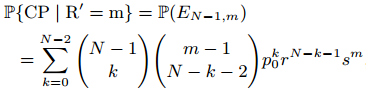
\includegraphics[width = 0.80\textwidth]{figs/cp.png}
	\end{subfigure}%
	\begin{subfigure}{0.50\textwidth}
	  \centering
	  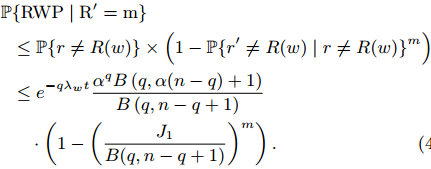
\includegraphics[width = 0.80\textwidth]{figs/rwp.png}
	\end{subfigure}
  \end{figure}
\end{frame}
%%%%%%%%%%%%%%%
\begin{frame}{PA2AM 量化分析}
  带时间的球盒模型, 计算 $\mathbb{P}(\textrm{RWP}|\textcolor{red}{\textrm{CP}})$:
	\begin{description}
	  \item<3->[建模目的:] $\mathbb{P}\set{R(r) = w'}$ ($R(r) \neq w$)
	  \item<4->[系统协议:] $n$ 副本节点; ``过半数'' {\small ($M = \lfloor n / 2 \rfloor + 1$)} 通信规则
	  \item<5->[球盒模型:] 操作产生 $n$ 个球, 发送到 $n$ 个副本盒子
	  \item<6->[时刻$t$:] 操作 $r$ \textcolor{brown}{恰好前 $M$ 个球}到达相应盒子
	  \item<7->[$R(r) \neq w$:] 操作 $w$ 相应 $M$ 个球尚在途中 
	  \item<8->[带时间:] 操作起始时间 + 消息延迟
	\end{description}

  \begin{figure}[h!]
    \centering
    \begin{adjustbox}{max totalsize = {0.50\textwidth}{1.00\textheight}, center}
      % new command: interval
\newcommand{\itv}[4]{ % #1: start point; #2: end point; #3: operation name; #4: style
  \coordinate (start #3) at #1;	% start point
  \coordinate (end #3) at #2;	% end point

  \draw[#4, |-|] (start #3) -- (end #3) % draw the interval
    node[pos = 0.5, above = 1mm,font = \Large, text=black] (#3) {$#3$}; % attach the operation name
}

\begin{tikzpicture}[
  comm/.style = {>=Stealth, <->, blue, very thick}, 
  nocomm/.style = {thick, dashed},
  noack/.style = {>=Stealth, ->, thick, blue, dashed}]

  % ops: w', w, and r
  \uncover<2->{
	\itv{(0,0)}{(2,0)}{w'}{ultra thick, blue}
	\itv{(4,0)}{(6,0)}{w}{ultra thick, blue}
	\itv{(5.5,-4)}{(7.5,-4)}{r}{very thick, brown}
  }

  % read-from relation
  \only<3>{
	\draw [dashed, line width = 2pt, gray, >=Stealth, ->] (w') to [out = -60, in = 100] (r.east);
  }

  % 3 replias (modeled as bins)
  \uncover<4->{
	\foreach \x in {1, 3, 5} {
	  \node (\x) [rectangle, double, draw, minimum size = 0.50cm] at (\x, -2) {};
	}
  }

  % w' sends balls into bins
  \uncover<5->{
	\draw[nocomm] (start w') to (1);
	\draw[comm] (start w') to (3);
	\draw[comm] (start w') to (5);
  }

  % r sends balls into bins
  \uncover<6->{
	\draw[noack, brown] (start r) to (1);
	\draw[nocomm] (start r) to (3);
	\draw[noack, brown] (start r) to (5);
  }

	% w sends balls into bins
  \uncover<7->{
	\draw[noack, shorten >= 8pt] (start w) to (1);
	\draw[nocomm] (start w) to (3);
	\draw[noack, shorten >= 8pt] (start w) to (5);
  }
\end{tikzpicture}
    \end{adjustbox}
  \end{figure}
\end{frame}
%%%%%%%%%%%%%%%
\begin{frame}{PA2AM 量化分析}
  \begin{figure}
	\begin{subfigure}{0.40\textwidth}
	  \centering
	  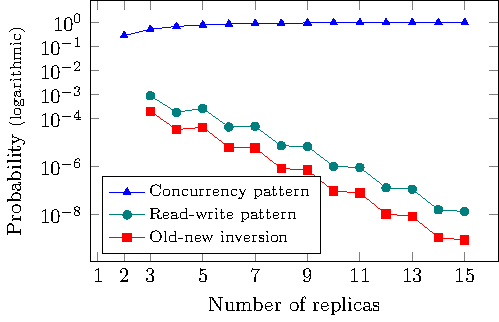
\includegraphics[width = 0.80\textwidth]{figs/oni-pgfplot.pdf}
	  \caption{数值结果.}
	\end{subfigure}%
	\begin{subfigure}{0.60\textwidth}
	  \centering
	  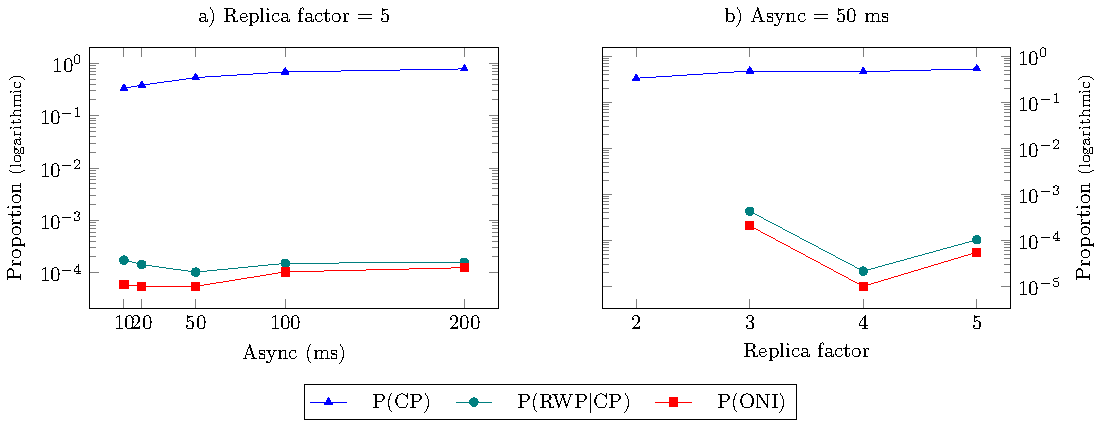
\includegraphics[width = 0.95\textwidth]{figs/experiment-oni-pgfplot.pdf}
	  \caption{实验结果.}
	\end{subfigure}
  \end{figure}

  \only<2->{
  \begin{cobservation}[观察一]
	从概率角度讲, PA2AM 算法极少违反 atomicity 一致性.
  \end{cobservation}
  }

  \only<3->{
  \begin{cobservation}[观察二]
	与经常发生的并发模式相比, 读写模式起主导作用。
  \end{cobservation}
}
\end{frame}
%%%%%%%%%%%%%%%
\begin{frame}{PA2AM vs. 弱一致性模型}
  \begin{figure}
	\begin{subfigure}{0.50\textwidth}
	  \centering
	  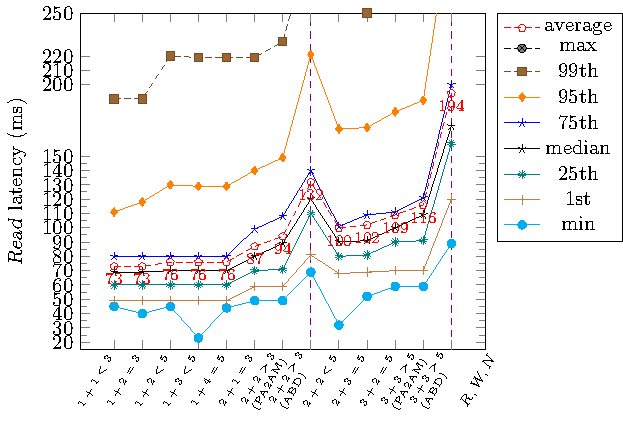
\includegraphics[width = 0.85\textwidth]{figs/rwn-2am-read-latency-quantiles.pdf}
	  \caption{读操作延迟对比.}
	\end{subfigure}%
	\begin{subfigure}{0.50\textwidth}
	  \centering
	  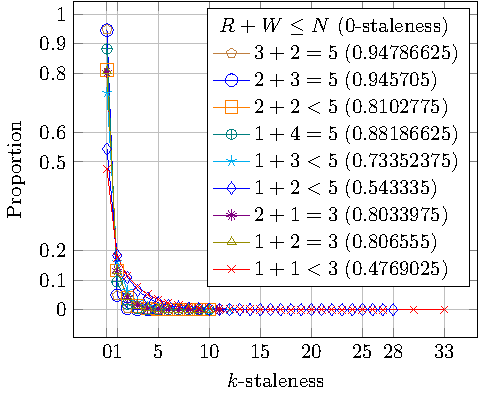
\includegraphics[width = 0.70\textwidth]{figs/rwn-maj.pdf}
	  \caption{$k$-陈旧度对比.}
	\end{subfigure}
	\caption{PA2AM 与 eventual consistency (RWN-Maj 协议) 对比结果.}
  \end{figure}

  \vspace{-0.50cm}
  \begin{table}[]
  \renewcommand{\arraystretch}{1.3}
  \centering
  \caption{不同 $R,W,N$ 配置下, RWN-All 执行中具有不同陈旧度的读操作的比率.}
  \label{tbl:rwn-all-staleness}
  \resizebox{\textwidth}{!}{%
  \begin{tabular}{|c||c|c|c|c||c|c|c|c|c|c|c|}
  \hline
  {\bfseries \# replicas} & \multicolumn{4}{c||}{\bfseries replica factor = 3 ($400,000$
    \textsl{read} operations)} & \multicolumn{7}{c|}{\bfseries replica factor = 5 ($800,000$
    \textsl{read} operations)} 
  \\ \hline
  {\bfseries $R,W,N$} % \textrm{R}+\textrm{W} $\boldsymbol{\le}$ \textrm{N}}  
  & $1+1<3$	& $1+2=3$	& $2+1=3$	& $2+2>3 \;(\text{PA2AM})$ 
  & $1+2<5$ 	& $1+3<5$ 	& $1+4=5$	& $2+2<5$ 	& $2+3=5$    & $3+2=5$     & $3+3>5 \;(\text{PA2AM})$     
  \\ \hline \hline
  {\boldmath $\max k$}          & $6$      & $4$ 	& $2$    &  {\boldmath $1$}
  & $2$	& $2$      	& $2$	   & $2$	& $2$	 &  $2$     & {\boldmath $1$}
  \\ \hline
  {\bfseries $\sum_{k \ge 1}$-staleness}       & $0.0084125$      & $0.000315$ 	&  $0.0004675$	&
  {\boldmath $0.000085$}
  	&  $0.00377875$	&  $0.002755$	&  $0.00406$     & $0.0027225$      & $0.0020275$     & $0.002255$      
	&  {\boldmath $0.0003525$}
  \\ \hline
  \end{tabular}%
}
\end{table}

\end{frame}
%%%%%%%%%%%%%%%
\begin{frame}{PA2AM 的意义}
  \mdf{red}{blue}{PA2AM 可作为数据一致性/访问延迟权衡的一种可行选项}{
	\begin{enumerate}
	  \item 既 {\small (在大多数时候)} 满足强一致性模型对数据一致性的高标准
	  \item 又具有弱一致性模型的性能优势
    \end{enumerate}
  }

  \pause
  \vspace{0.30cm}

  \mdf{red}{blue}{PA2AM 在相关工作中的意义}{
	\begin{enumerate}
	  \item {\textcolor{gray}{\small (AFAWK)}} \textcolor{red}{首次} ``确定性陈旧度有界 + 概率'' \\
		\citeinbeamer{Aiyer}{DISC}{05} \citeinbeamer{Lee}{DC}{05} \citeinbeamer{Bailis}{PVLDB}{12}
	  \item 度量违反 \textcolor{red}{atomicity} {\small (vs. regularity \citeinbeamer{Lee}{DC}{05} \citeinbeamer{Bailis}{PVLDB}{12})} 的程度
    \end{enumerate}
  }
\end{frame}
%%%%%%%%%%%%%%%

% file: sections/vpc.tex

\subsection{VPC: Pipelined-RAM 一致性验证}

\newcommand{\pram}{Pipelined-RAM}
\newcommand{\PRAM}{PRAM}
\newcommand{\vpc}[1]{\ifthenelse{\isempty{#1}{}}{\textsf{VPC}}{\textsf{VPC-\MakeUppercase{#1}}}} 
\newcommand{\npc}{$\sf{NP}$-complete}
\newcommand{\npcn}{$\sf{NP}$-completeness}
\newcommand{\rwclosure}{\textsc{RW-Closure}}
\newcommand{\readcentric}{\textsc{Read-Centric}}

%%%%%%%%%%%%%%%
\begin{frame}{}
  \fignocaption{width = 0.65\textwidth}{figs/rdt-research-vpc}
\end{frame}
%%%%%%%%%%%%%%%

% file: sections/vpc-work.tex

%%%%%%%%%%%%%%%
\begin{frame}{}
  \begin{center}
    \vspace{0.50cm}
    协议验证 (Verification of a Protocol) \\[5pt]
    \ncite{Bouajjani:POPL14} \ncite{Bouajjani:POPL17}

    \vspace{0.30cm}
    \hl{执行验证 (Verification of an Execution)}

    \pause
    \vspace{0.50cm}

    \fignocaption{width = 0.50\textwidth}{figs/sla}
    
    \vspace{0.30cm}
    {黑盒测试/确认系统是否提供了其所声称的数据一致性}

    \ncite{Amazon:SOSP07} \ncite{Golab:PODC11}
  \end{center}
\end{frame}
%%%%%%%%%%%%%%%

%%%%%%%%%%%%%%%
\begin{frame}{}
  \begin{description}
    \item[\red{\large PRAM:}] 包含存储系统常提供的最基本的``会话'' \term{session} 一致性

	\ncite{Terry:PDIS94} \ncite{Brzezinski:PDP04}
  \end{description}

  \fignocaption{width = 0.60\textwidth}{figs/pram-monotonic-writes-example}
  \vspace{-0.10cm}
  {\centerline{\PRAM{} 保证``单调写''性质}}
\end{frame}
%%%%%%%%%%%%%%%

%%%%%%%%%%%%%%%
\begin{frame}{}
  \begin{cdef}[VPC (Verifying PRAM Consistency) 判定问题]
    \vspace{8pt}
    \begin{description}
      \setlength{\itemsep}{8pt}
      \item[实例:] 系统执行 \emph{\small (execution $e$)}
      \item[问题:] 该执行 $e$ 是否满足 \emph{PRAM} 一致性模型 \emph{\small ($\mathcal{C}$)}? 
    \end{description}    

    \[
      e \in \mathcal{C} \Rightarrow \set{0,1}?
    \]
  \end{cdef}
\end{frame}
%%%%%%%%%%%%%%%

%%%%%%%%%%%%%%%
\begin{frame}{}
  \begin{cdef}[系统执行]
    系统执行 $e \triangleq \{h_p \mid h_p: \text{进程 } \;p \text{ 上的读写操作序列}\}$

    \vspace{0.30cm}
    \textcolor{blue}{规模 $n$:} 系统执行中读写操作的总数
  \end{cdef}

  \vspace{0.50cm}
  \fignocaption{width = 0.70\textwidth}{figs/execution-example.pdf}
\end{frame}
%%%%%%%%%%%%%%%

%%%%%%%%%%%%%%%
\begin{frame}{}
  \begin{cdef}[\PRAM{} 一致性模型]
    \begin{center}
      系统执行 $e$ 满足 \emph{\PRAM{}} 一致性 \\[5pt]
      $\iff$ \\[5pt]
      $\forall p:$ $p$ 上\textcolor{blue}{所有操作}与其它进程上所有\textcolor{blue}{写操作}存在\textcolor{red}{合法}调度
    \end{center}
  \end{cdef}

  \vspace{0.30cm}
  % \fignocaption{width = 0.65\textwidth}{figs/execution-example.pdf}
  \begin{center}
    \resizebox{0.65\textwidth}{!}{\input{tikz/execution-example}}
  \end{center}

  \pause
  \vspace{-0.80cm}

  \begin{gather*}
    p_{0}: Wf2\; Wf1\; Wz2\; \textcolor<3>{blue}{Wz1}\; Wy2\; Wy1\; \textcolor{brown}{Rf1} 
    Wx5\; Wx3\; \textcolor<4>{red}{Wx2}\; Wc1\; \textcolor{brown}{Rc1} \\
    \textcolor{brown}{Rz1} \textcolor{brown}{Ry1}
    Wa1\; \textcolor{brown}{Ra1} \textcolor<3>{blue}{Wb1}\; \textcolor{brown}{Rb1} \textcolor<4>{red}{\textcolor<1-3>{brown}{Rx2}}
  \end{gather*}
\end{frame}
%%%%%%%%%%%%%%%

%%%%%%%%%%%%%%%
\begin{frame}{}
  \begin{table}[!t]
    \centering
    \caption{VPC 问题的四种变体 (按``执行''的类型) 及复杂度 \\ \red{\small ($[\ast]:$ 本文工作)}}
    \renewcommand\arraystretch{1.2}
    \resizebox{\textwidth}{!}{%
      \begin{tabular}{|c|c|c|}
	\hline
	& \it (S)ingle variable  & \it (M)ultiple variables
	\\ \hline
	    {\it write (D)uplicate values} &
	    \innercell{c}{VPC-SD \\ \uncover<2->{\textcolor{red}{\small (\npc{}) $[\ast]$}}} &
	    \innercell{c}{VPC-MD \\ \uncover<2->{\textcolor{red}{\small (\npc{}) $[\ast]$}}}
	\\ \hline
	    \only<1-2>{\it write (U)nique value}\only<3>{\cellcolor{brown!80}{\it write (U)nique value}} &
	    \innercell{c}{VPC-SU \\ \uncover<2->{\textcolor{blue}{\small (P)}} \\ \uncover<2->{\ncite{Golab:PODC11}}} &
	    \innercell{c}{VPC-MU \\ \uncover<2->{\textcolor{red}{\small (P) $[\ast]$}}}
	\\ \hline
      \end{tabular}
    }
  \end{table}

  \vspace{10pt}
  \uncover<3->{\textcolor{brown}{\centerline{Read-mapping \ncite{Gibbons:SICOMP97}: $\forall r,\; \exists! w,\; f(r) = w$.}}}
\end{frame}
%%%%%%%%%%%%%%%

%%%%%%%%%%%%%%%
\begin{frame}{}
  \begin{center}
    \hl{\large VPC-SD (VPC-MD) 是 \npc{} 问题}
  \end{center}
  % 多项式归约: 从 \textsc{Unary 3-Partition} 到 \vpc{sd}

  \pause
  \fig{width = 0.40\textwidth}{figs/vpcsd-npc}
  {\textsc{Unary 3-Partition} 实例 $A = \{2,2,1,1,1,1\}, m = 2, B = 4$ 对应的 VPC-SD 执行} 
\end{frame}
%%%%%%%%%%%%%%%

%%%%%%%%%%%%%%%
\begin{frame}{}
  \begin{center}
    \fignocaption{width = 0.40\textwidth}{figs/mdb-stack}

    \pause
    \vspace{0.40cm}
    \begin{quote}
      ``Basically I'm a programmer :-)  \\[8pt] \pause

      I enjoy reading papers about the complexity of puzzle games, \\[2pt]

      and I'm writing (amateur) proofs on the complexity of a few puzzle games.''
    \end{quote}

    \pause
    \vspace{0.30cm}
    \fignocaption{width = 0.90\textwidth}{figs/nearly42}
  \end{center}
\end{frame}
%%%%%%%%%%%%%%%

%%%%%%%%%%%%%%%
\begin{frame}{}
  \begin{center}
    {\hl{\large VPC-MU 的多项式算法 \rwclosure{}}}
  \end{center}

  \begin{figure}[h!]
    \centering
    \begin{adjustbox}{max totalsize = {0.60\textwidth}{1.00\textheight}, center}
      \input{tikz/rw-closure-example}
    \end{adjustbox}
    \caption{\rwclosure{} 算法示例: 在传递闭包之上迭代应用 $w'wr$ 规则}
  \end{figure}

  \vspace{-0.30cm}
  \uncover<4->{\fignocaption{width = 0.25\textwidth}{figs/wprimewr-order.pdf}}
\end{frame}
%%%%%%%%%%%%%%%

%%%%%%%%%%%%%%%
\begin{frame}{}
  \begin{ctheorem}[\rwclosure{} 算法正确性]
    \begin{center}
      \emph{\vpc{mu}} 实例满足 \emph{\PRAM{}} 一致性 \\[5pt]
      $\iff$ \\[5pt]
      \rwclosure{} 算法所得图是 \emph{DAG} 图
    \end{center}
  \end{ctheorem}

  \pause
  \vspace{0.20cm}

  \begin{cproof}
    \begin{description}
      \item[``$\Longrightarrow$''] 反证法
      \item[``$\Longleftarrow$''] \hl{对读操作作数学归纳}, 构造合法调度
    \end{description}
  \end{cproof}

  \pause
  \vspace{0.50cm}
  \rwclosure{} 算法复杂度: 
  \[
    \underbrace{O(n^2)}_{\textrm{\#loops}} \quad\cdot
	\underbrace{O(n^3)}_{\textrm{transitive closure}}  = O(n^5)
  \]
\end{frame}
%%%%%%%%%%%%%%%

%%%%%%%%%%%%%%%
\begin{frame}{}
  \rwclosure{} 算法的缺点:
  \begin{itemize}
	\item 在全图上应用 $w'wr$ 规则
	\item 应用 $w'wr$ 规则无特定顺序
  \end{itemize}

  \pause
  \vspace{0.80cm}

  \hl{VPC-MU 的多项式算法 \readcentric{} 要点:}
  \begin{itemize}
    \item \textcolor{blue}{增量式}调度每个读操作
    \item 在读操作诱导的\textcolor{blue}{局部子图}上按\textcolor{blue}{逆拓扑序}应用 $w'wr$ 规则
  \end{itemize}
\end{frame}
%%%%%%%%%%%%%%%

%%%%%%%%%%%%%%%
\begin{frame}{}
  \begin{ctheorem}[\readcentric{} 算法正确性]
    \begin{center}
      \emph{\vpc{mu}} 实例满足 \emph{\PRAM{}} 一致性 \\[5pt]
      $\iff$ \\[5pt]
      \readcentric{} 算法所得图是 \emph{DAG} 图
    \end{center}
  \end{ctheorem}

  \pause
  \vspace{0.30cm}
  \begin{cproof}
    \[
      \readcentric{}\;\; \purple{\xLeftrightarrow{\quad Reachability \quad}} \;\;\rwclosure{}
    \]
  \end{cproof}

  \pause
  \vspace{0.60cm}
  \readcentric{} 算法复杂度: 
  \[
    \underbrace{O(n)}_{\textrm{\blue{\#reads}}} \cdot
    \underbrace{O(n \cdot n^2)}_{\red{\textsc{Topo-Schedule}}} = O(n^4)
  \]
\end{frame}
%%%%%%%%%%%%%%%

% file: sections/vpc-related.tex

%%%%%%%%%%%%%%%
% \begin{frame}{}
%   \mdf{red}{blue}{VPC 在相关工作中的意义}{
%     \hl{较早关注} {\small (分布式系统领域)} ``弱一致性模型验证''问题 {\small (\hl{\red{2013$\sim$}})}:
%     \begin{description}
%       \setlength{\itemsep}{6pt}
%       \item[强一致性:] \ncite{Gibbons:SICOMP97} \ncite{Cantin:TPDS05} \ncite{Golab:PODC11} 
%       \item[弱一致性:] \ncite{Furbach:ACSD14} \ncite{Bouajjani:POPL17} \\ \ncite{Emmi:CAV18}
%     \end{description}
%   }
% \end{frame}
%%%%%%%%%%%%%%%

%%%%%%%%%%%%%%%
\begin{frame}{}
  \begin{table}[h]
    \centering
    \caption{{\bf VSC} (Verifying Sequential Consistency) 与 {\bf VL} (Verifying Linearizability) 问题的复杂度~\ncite{Gibbons:SICOMP97}}
    \renewcommand\arraystretch{1.2}
    % \resizebox{\textwidth}{!}{
      \begin{tabular}{|c|c|c|}
	\hline
	{\bf Variants} & {\bf VSC} & {\bf VL}
	\\ \hline \hline
	\hl{\red{General}} & \textsf{NP}-complete & \textsf{NP}-complete
	\\ \hline
	$2$ Operations/Process & \textsf{NP}-complete & \textsf{NP}-complete
	\\
	$2$ Variables & \textsf{NP}-complete & \textsf{NP}-complete \\
	$3$ Processes & \textsf{NP}-complete & $O(n \log n)$
	\\ \hline
	Read-mapping & \textsf{NP}-complete &  $O(n \log n)$ \\
	Write-order & \textsf{NP}-complete &  $O(n \log n)$ \\
	\texttt{read\&write} only & \textsf{NP}-complete & \textsf{NP}-complete \\
	Conflict-order & $O(n \log n)$ &  $O(n \log n)$
	\\ \hline
      \end{tabular}
    % }
  \end{table}
\end{frame}
%%%%%%%%%%%%%%%

%%%%%%%%%%%%%%%
\begin{frame}
  \begin{table}[h]
    \centering
    \caption{{\bf VMC} (Verifying Memory Coherence) 问题的复杂度~\ncite{Cantin:TPDS05}}
    % \renewcommand\arraystretch{1.1}
    \resizebox{\textwidth}{!}{
      \begin{tabular}{|c|c|c|}
	\hline
	{\bf Variants} & {\bf \texttt{\bf Read/Write}} & {\bf \texttt{\bf Read-Modify-Write}}
	\\ \hline \hline
	$1$ Operation/Process & $O(n \lg n)$ & $O(n^2)$ \\
	$2$ Operations/Process & ? & \textsf{NP}-complete \\
	$3+$ Operations/Process & \textsf{NP}-complete & \textsf{NP}-complete
	\\ \hline
	Constant $k$ processes & $O(n^k)$ & $O(n^k)$
	\\ \hline
	\innercell{c}{$1$ Write/Value \\ {\small (Read-mapping)}} & $O(n)$ & $O(n \lg n)$ \\
	$2$ Writes/Value & \textsf{NP}-complete & ? \\
	$3+$ Writes/Value & \textsf{NP}-complete & \textsf{NP}-complete
	\\ \hline
	Write-order & $O(n^2)$ & $O(n)$
	\\ \hline
      \end{tabular}
    }
  \end{table}
\end{frame}
%%%%%%%%%%%%%%%

%%%%%%%%%%%%%%%
\begin{frame}{}
  \begin{table}[h]
    \centering
    \caption{{\bf Atomicity}~\footnote{也称 Linearizability} 相关一致性模型验证问题复杂度 {\small (假设: 不允许写重复值)}}
    \renewcommand\arraystretch{1.1}
    \resizebox{\textwidth}{!}{
      \begin{tabular}{|c|c|c|c|c|}
	\hline
	& \textbf{Safety} & \textbf{Regularity} & \textbf{Atomicity} & \textbf{Sequential}
	\\ \hline  \hline
	\begin{tabular}[c]{@{}c@{}}
	  \textbf{Offline}\\ \ncite{Anderson:HotDep10}
	\end{tabular}
	& $O(n^2)$ & $O(n^2)$ & $O(n^3)$ & {\it not studied}
	\\ \hline
	\begin{tabular}[c]{@{}c@{}}\textbf{Online}~\footnote[frame]{包含其它假设}\\
	\ncite{Golab:PODC11} \end{tabular} 
	& $O(n)$ & $O(n)$ & $O(n \log n)$ & $\textsf{Poly}(n)$
	\\ \hline
      \end{tabular}
    }
  \end{table}
\end{frame}
%%%%%%%%%%%%%%%

%%%%%%%%%%%%%%%
\begin{frame}{}
  \begin{table}
    \centering
    \caption{$k$-AV {\small ($k$-Atomicity Verification)} 问题复杂度}
    \renewcommand\arraystretch{1.4}
    \resizebox{\textwidth}{!}{
      \begin{tabular}{|c|c|c|c|}
	\hline
	{\bf Problems} & {\bf Variants} 	& {\bf Results} 	& {\bf Work} 				\\ \hline \hline
	$1$-AV	&	General			&	\npc{}		&	\ncite{Gibbons:SICOMP97}	\\ \hline
	$1$-AV	&	Write unique value	&	$O(n \log n)$	&	\ncite{Gibbons:SICOMP97}	\\ \hline		
	$2$-AV	&	Write unique value	&	$O(n \log n)$	&	\ncite{Golab:ICDCS13}		\\ \hline
	$k$-AV	&	\innercell{c}{Write unique value \\ Bounded concurrency}	&	$O(n^2)$	
		&	\innercell{c}{\ncite{Golab:PODC15} \\ \ncite{Golab:SICOMP18}}				\\ \hline
    \hl{$k$-AV} & \hl{\red{Write unique value}}
		& \only<2->{
		    \begin{minipage}{0.25\textwidth}
		      
\includegraphics[width = \linewidth]{figs/dont-know-panda}
		    \end{minipage} }	
		& \only<3->{
		    \begin{minipage}{0.2\textwidth}
		      
\includegraphics[width = \linewidth]{figs/waiting-bear}
		    \end{minipage} } \\ \hline
      \end{tabular}
    }
  \end{table}
\end{frame}
%%%%%%%%%%%%%%%

%%%%%%%%%%%%%%%
\begin{frame}{}
  % \centerline{直观地说, 每个操作 {\small (\textcolor{blue}{区间})} 都如同瞬时 {\small (\textcolor{blue}{点})} 发生的一样。}
  \begin{center}
    \hl{\large Atomicity = 实时序 + 读写语义} \\[5pt]

    \ncite{Lamport:DC86}
  \end{center}

  \vspace{0.20cm}
  \begin{center}
    \resizebox{0.60\textwidth}{!}{\input{tikz/atomicity-example}}
  \end{center}
\end{frame}
%%%%%%%%%%%%%%%

%%%%%%%%%%%%%%%
\begin{frame}{}
  \begin{center}
    \hl{\large $k$-Atomicity = 实时序 + $k$-读写语义} \\[5pt]
    
    \ncite{Aiyer:DISC05} \ncite{Taubenfeld:ICDCN13}
  \end{center}

  \vspace{0.20cm}
  \begin{center}
    \resizebox{0.75\textwidth}{!}{\input{tikz/katomicity-trace-not12atomic}}
  \end{center}

  \uncover<3->{
    \[ 
      3\text{-Atomicity}: w5\quad \red{w2}\quad w1\quad r1\quad w3\quad w4\quad \red{r2}\quad r3\quad r4 
    \]
  }
\end{frame}
%%%%%%%%%%%%%%%

%%%%%%%%%%%%%%%
\begin{frame}{}
  \begin{cdef}[$k$-AV {\small ($k$-Atomicity Verification)} 判定问题]
    \vspace{8pt}
    \begin{description}
      \setlength{\itemsep}{8pt}
      \item[实例:] 系统执行 $e$ \blue{\small \emph{(不允许写重复值)}}、参数 $k$
      \item[问题:] 该执行 $e$ 是否满足 $k$\emph{-Atomicity?}
    \end{description}
  \end{cdef}
\end{frame}
%%%%%%%%%%%%%%%


%%%%%%%%%%%%%%%

% file: sections/future.tex

\section{未来工作}

%%%%%%%%%%%%%%%
\begin{frame}{}
  \fignocaption{width = 0.618\textwidth}{figs/one-more-thing}
\end{frame}
%%%%%%%%%%%%%%%

%%%%%%%%%%%%%%%
\begin{frame}{}
  \fignocaption{width = 0.65\textwidth}{figs/rdt-research-spec}
\end{frame}
%%%%%%%%%%%%%%%

%%%%%%%%%%%%%%%
\begin{frame}{}
  \begin{center}
    \uncover<2->{\hl{\large 规约: 数据一致性模型 (Consistency Model)}}
  \end{center}

  \begin{columns}
    \column{0.50\textwidth}
      \begin{center}
	多处理器系统中的并发数据类型
      \end{center}
      \vspace{0.60cm}
      \fignocaption{width = 0.50\textwidth}{figs/cdt}
    \column{0.50\textwidth}
      \begin{center}
	分布式系统中的复制数据类型
      \end{center}
      \fignocaption{width = 0.60\textwidth}{figs/rdt}
  \end{columns}

  \vspace{0.20cm}
  \uncover<3->{
    \begin{center}
      \red{\LARGE PL + DC \uncover<4->{+ FM}}	\ncite{Burckhardt:POPL14}
    \end{center}
  }
\end{frame}
%%%%%%%%%%%%%%%


\thankyou{}
% file: panel.tex

%%%%%%%%%%%%%%%
\begin{frame}[noframenumbering]
  \begin{enumerate}[(I)]
    \setlength{\itemsep}{15pt}
    \item {\large DC + PL + FM:}
      \begin{itemize}
	\setlength{\itemsep}{6pt}
	\item 有哪些问题可以共享?
	\item 有哪些理论、技术可以相互借鉴?
	\item 分布式系统中的编程模型?
	\item 并发数据类型的验证技术应用于复制数据类型?
	\item 分布式系统中的数据一致性模型 \emph{vs.} 多处理器系统中的内存模型?
	\item $\cdots$
      \end{itemize}
    \item {研究经验分享:}
      \begin{itemize}
	\setlength{\itemsep}{6pt}
	\item 如何选择研究问题?
	\item 给青年学者的建议
	\item $\cdots$
      \end{itemize}
  \end{enumerate}
\end{frame}
%%%%%%%%%%%%%%%


% file: sections/appendix.tex

\section{附录}

\appendix

% file: sections/bib.tex

%%%%%%%%%%%%%%%%%%%%
\begin{frame}[allowframebreaks]
  \printbibliography
\end{frame}
%%%%%%%%%%%%%%%%%%%%


%%%%%%%%%%%%%%%%%%%% Begin: Jupiter %%%%%%%%%%%%%%%%%%%%

%%%%%%%%%%%%%%%%%%%%
\begin{frame}{}
  \centerline{\large 针对列表的操作转换函数~\ncite{Ellis:SIGMOD89}}

  \resizebox{\textwidth}{!}{
    \begin{minipage}{\textwidth}
      % file: parts/list-ot.tex

\newcommand{\ldel}{\textsc{Del}}	% List DEL
\newcommand{\lins}{\textsc{Ins}}	% List INS
\newcommand{\ldelop}[2]{\ldel\left(#1, #2\right)}  % #1: index, #2: priority
\newcommand{\linsop}[3]{\lins\left(#1, #2, #3\right)}  % #1: index, #2: element, #3: priority

%%%%%%%%%% list-ot.tex %%%%%%%%%% 
\begin{align*}
  % ins vs. ins
  OT\Big(\lins(a_1, p_1, pr_1), \lins(a_2, p_2, pr_2)\Big) &= \begin{cases}
    \lins(a_1, p_1, pr_1) 		& p_1 < p_2 \\[3pt]
    \lins(a_1, p_1 + 1, pr_1) 		& p_1 > p_2 \\[3pt]
    \textsc{NOP} 			& p_1 = p_2 \land a_1 = a_2 \\[3pt]
    \lins(a_1, p_1 + 1, pr_1) 		& p_1 = p_2 \land a_1 \neq a_2 \land pr_1 > pr_2 \\[3pt]
    \lins(a_1, p_1, pr_1)		& p_1 = p_2 \land a_1 \neq a_2 \land pr_1 \le pr_2
  \end{cases} \\[10pt]
  % ins vs. del
  OT\Big(\lins(a_1, p_1, pr_1), \ldel(\_, p_2, pr_2)\Big) &= \begin{cases}
    \lins(a_1, p_1, pr_1) 		& p_1 \le p_2 \\[3pt]
    \lins(a_1, p_1 - 1, pr_1) 		& p_1 > p_2
  \end{cases} \\[10pt]
  % del vs. ins
  OT\Big(\ldel(\_, p_1, pr_1), \lins(a_2, p_2, pr_2)\Big) &= \begin{cases}
    \ldel(\_, p_1, pr_1) 		& p_1 < p_2 \\[3pt]
    \ldel(\_, p_1 + 1, pr_1) 		& p_1 \ge p_2
  \end{cases} \\[10pt]
  % del vs. del
  OT\Big(\ldel(\_, p_1, pr_1), \ldel(\_, p_2, pr_2)\Big) &= \begin{cases}
    \ldel(\_, p_1, pr_1) 		& p_1 < p_2 \\[3pt]
    \ldel(\_, p_1 - 1, pr_1) 		& p_1 > p_2 \\[3pt]
    \textsc{NOP}			& p_1 = p_2
  \end{cases} \\
\end{align*}
%%%%%%%%%% list-ot.tex %%%%%%%%%% 

    \end{minipage}
  }
\end{frame}
%%%%%%%%%%%%%%%%%%%%
%%%%%%%%%%%%%%%%%%%% End: Jupiter %%%%%%%%%%%%%%%%%%%%

%%%%%%%%%%%%%%%%%%%% Begin: VPC %%%%%%%%%%%%%%%%%%%%

%%%%%%%%%%%%%%%
\begin{frame}{}
  \begin{ctheorem}[\rwclosure{} 算法正确性]
    \begin{center}
      \emph{\vpc{mu}} 实例满足 \emph{\PRAM{}} 一致性 \\[5pt]
      $\iff$ \\[5pt]
      \rwclosure{} 算法所得图是 \emph{DAG} 图
    \end{center}
  \end{ctheorem}

  \pause
  \vspace{0.20cm}

  \begin{cproof}
    \begin{description}
      \item[``$\Longrightarrow$''] 反证法
      \item[``$\Longleftarrow$''] 
	\textcolor{red}{难点:} DAG 图蕴含着多个全序

	\textcolor{red}{技巧:} 对读操作作数学归纳, 构造合法调度
    \end{description}
  \end{cproof}

  \pause
  \vspace{0.30cm}

  \rwclosure{} 算法复杂度: 
  \[
    \underbrace{O(n^2)}_{\textrm{\#loops}} \quad\cdot
	\underbrace{O(n^3)}_{\textrm{transitive closure}}  = O(n^5)
  \]
\end{frame}
%%%%%%%%%%%%%%%

%%%%%%%%%%%%%%%
\begin{frame}{}
  \readcentric{} 算法复杂度: 
  \[
    \underbrace{O(n)}_{\textrm{iterations}} \cdot
	\underbrace{O(n \cdot n^2)}_{\textcolor{red}{\textsc{Topo-Schedule}}} = O(n^4)
  \]

  \vspace{0.30cm}
  \begin{clemma}[\textsc{Topo-Schedule} 的非迭代性]
    \begin{center}
      设\textsc{Topo-Schedule} 正在处理读操作$r$,\\
      则\textcolor{blue}{局部子图}中的每个写操作\textcolor{red}{最多只有一次机会}\\
      在满足规则 $w'wr$ 的三元组中扮演``$w'$角色''。
    \end{center}
  \end{clemma}
\end{frame}
%%%%%%%%%%%%%%%

%%%%%%%%%%%%%%%
\begin{frame}{实验评估}
  实验目的~\footnotemark[1]~\footnotetext[1]{机器配置: Intel Core i7 3.40GHZ, 4GB RAM.}:
  \begin{enumerate}
    \item 考察 \readcentric{} 算法的实际效率 
      \textcolor{blue}{\small ({\it vs.} 渐近时间复杂度)}
    \item 对比 \readcentric{} 算法与 \rwclosure{} 算法的效率
  \end{enumerate}

  \pause
  \vspace{0.50cm}

  两类负载:
  \begin{enumerate}
    \item 随机生成的系统执行
    \item 满足 \PRAM{} 一致性的系统执行 \textcolor{red}{\small ($\approx$ 最坏情况输入)}
  \end{enumerate}
\end{frame}
%%%%%%%%%%%%%%%

%%%%%%%%%%%%%%%
\begin{frame}{}
  \begin{figure}[t]
    \centering
    \begin{subfigure}[t]{0.50\textwidth}
      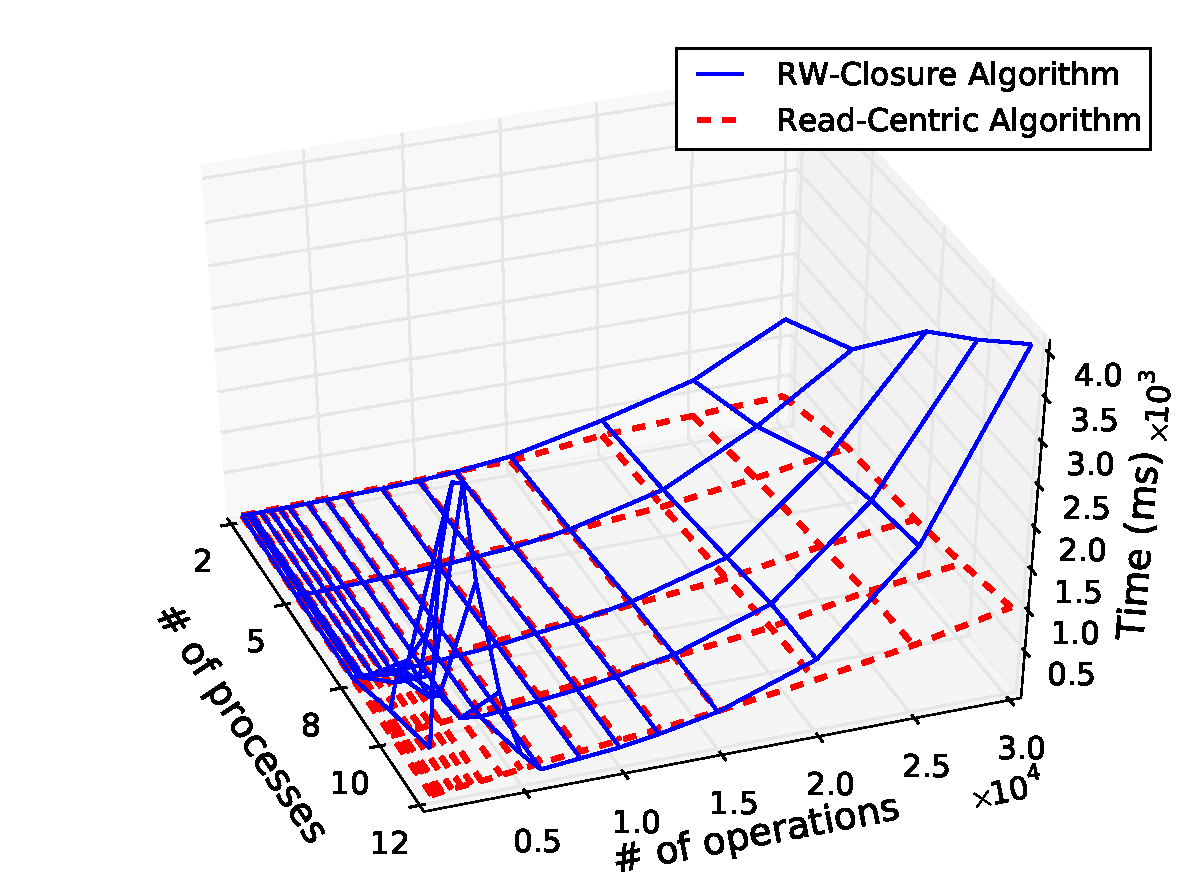
\includegraphics[width = 0.80\textwidth]{figs/vpc-random-cmp.pdf}
    \end{subfigure}%
    ~
    \begin{subfigure}[t]{0.50\textwidth}
      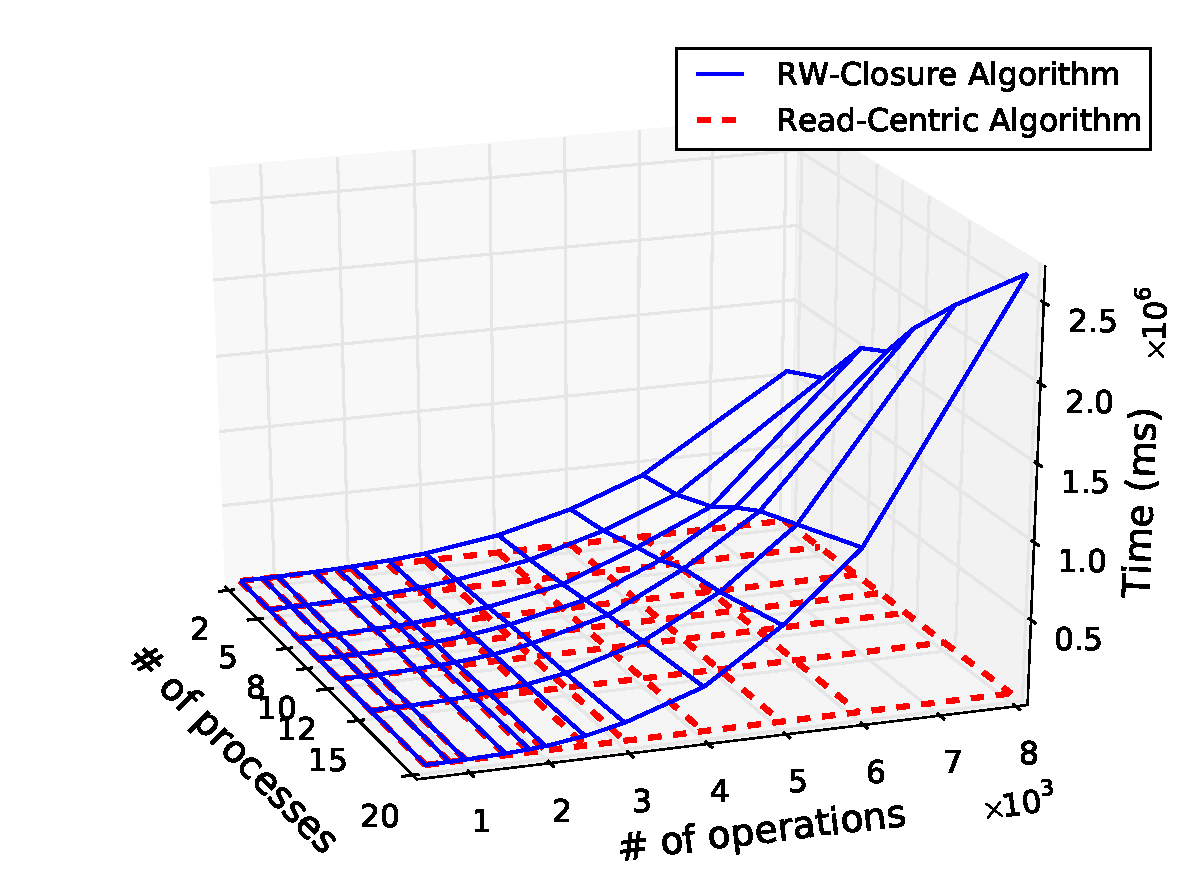
\includegraphics[width = 0.80\textwidth]{figs/vpc-valid-cmp.pdf}
    \end{subfigure}
    \caption{\rwclosure{} 算法与 \readcentric{} 算法在
    \textcolor{blue!80}{ (左) 随机生成}的执行及
    \textcolor{red!80}{ (右) 满足 \PRAM{} 一致性}的执行上的运行时间。}
  \end{figure}

  \pause
  \begin{center}
    \textcolor{red}{(右)} 20个进程、8,000 个操作: 

    \readcentric{} 可获得 694 倍加速.
  \end{center}
\end{frame}
%%%%%%%%%%%%%%%

%%%%%%%%%%%%%%%
\begin{frame}{}
  \fig{width = 0.45\textwidth}{figs/vpc-scalability-more.pdf}
  {\readcentric{} 算法在满足 \PRAM{} 一致性的执行上的运行时间}

  \vspace{-0.30cm}

  \begin{description}
    \centering
    \item[\readcentric{}:] 20个进程、60,000个操作 < 600s~\footnotemark[1]~\footnotetext[1]{用于测试, 规模可用}
    \item[\rwclosure{}:] 20个进程、8,000个操作 > 3,000s
  \end{description}
\end{frame}
%%%%%%%%%%%%%%%

%%%%%%%%%%%%%%%
\begin{frame}{}
  \begin{center}
    \hl{\large $\mathcal{I}$-Atomicity = $i$-实时序 + 读写语义}
  \end{center}

  \vspace{0.60cm}
  \centerline{$\mathcal{I}$: Inversions}

  \pause
  \vspace{0.30cm}
  \[
    f(\set{\text{inversions}}) \le i
  \]

  \pause
  \vspace{0.50cm}
  \centerline{\large 定义\red{框架}}
\end{frame}
%%%%%%%%%%%%%%%
%%%%%%%%%%%%%%%%%%%% End: VPC %%%%%%%%%%%%%%%%%%%%

%%%%%%%%%%%%%%%%%%%% Begin: Future Work %%%%%%%%%%%%%%%%%%%%
%%%%%%%%%%%%%%%
\begin{frame}{}
  \begin{center}
    ($50$种) \hl{一致性模型}关系图 \ncite{Viotti:CSUR16} \ncite{Burckhardt:Book14}
  \end{center}

  \fignocaption{width = 0.95\textwidth}{figs/non-transactional-consistency-models}

  \centerline{\red{\large 建立统一的形式化框架}}
\end{frame}
%%%%%%%%%%%%%%%%%%%% End: Future Work %%%%%%%%%%%%%%%%%%%%


\end{document}